\documentclass{subfile}
\begin{document}
\begin{figure}[!h]
    \centering
    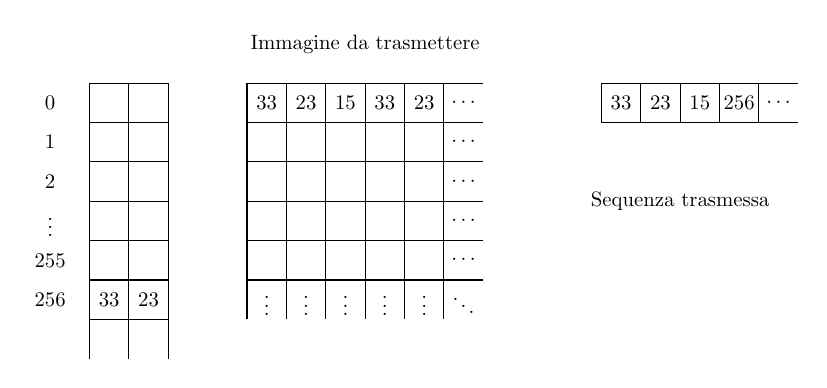
\begin{tikzpicture}[every node/.style={scale = 0.75}]

        \draw[step = 0.5] (0, 0) grid (2.5, -2.5);

        \foreach \i in {0, 0.5, ..., 2.5}{
                \draw (\i, -2.5) -- (\i, -3);
                \draw (2.5, - \i) -- (3, - \i);
            }

        \draw (1.5, 0.5) -- (1.5, 0.5) node {Immagine da trasmettere};

        \draw [step = 0.5] (-1, 0) grid (-2, -3);

        \foreach \i in {-1, -1.5, -2}{
                \draw (\i, -3) -- (\i, -3.5);
            }

        \foreach \i in {0.25, 0.75, ..., 2.25}{
                \draw (2.75, -\i) -- (2.75, -\i) node {\(\cdots\)};
                \draw (\i, -2.75) -- (\i, -2.75) node {\vdots};
            }

        \draw (2.75, -2.75) -- (2.75, -2.75) node {\(\ddots\)};

        \draw (-2.5, -0.25) -- (-2.5, -0.25) node {0};
        \draw (-2.5, -0.75) -- (-2.5, -0.75) node {1};
        \draw (-2.5, -1.25) -- (-2.5, -1.25) node {2};
        \draw (-2.5, -1.75) -- (-2.5, -1.75) node {\vdots};
        \draw (-2.5, -2.25) -- (-2.5, -2.25) node {255};
        \draw (-2.5, -2.75) -- (-2.5, -2.75) node {256};

        \draw (0.25, -0.25) -- (0.25, -0.25) node {33};
        \draw (0.75, -0.25) -- (0.75, -0.25) node {23};
        \draw (1.25, -0.25) -- (1.25, -0.25) node {15};
        \draw (1.75, -0.25) -- (1.75, -0.25) node {33};
        \draw (2.25, -0.25) -- (2.25, -0.25) node {23};

        \draw (-1.75, -2.75) -- (-1.75, -2.75) node {33};
        \draw (-1.25, -2.75) -- (-1.25, -2.75) node {23};

        \draw[step = 0.5] (4.5, 0) grid (6.5, -0.5);

        \foreach \i in {0, -0.5} {
                \draw (6.5, \i) -- (7, \i);
            }

        \draw (4.5, 0) -- (4.5, -0.5);

        \draw (6.75, -0.25) -- (6.75, -0.25) node {\(\cdots\)};

        \draw (5.5, -1.5) -- (5.5, -1.5) node {Sequenza trasmessa};

        \draw (4.75, -0.25) -- (4.75, -0.25) node {33};
        \draw (5.25, -0.25) -- (5.25, -0.25) node {23};
        \draw (5.75, -0.25) -- (5.75, -0.25) node {15};
        \draw (6.25, -0.25) -- (6.25, -0.25) node {256};

    \end{tikzpicture}
    \caption{Esempio di operatività dell'algoritmo di Lempel-Ziv-Welch.}
    \label{fig:6.1}
\end{figure}
\end{document}